\documentclass[conference]{IEEEtran}
\usepackage{cite}
\usepackage{amsmath,amssymb,amsfonts}
\usepackage{graphicx}
\usepackage{textcomp}
\usepackage{xcolor}
\def\BibTeX{{\rm B\kern-.05em{\sc i\kern-.025em b}\kern-.08em
    T\kern-.1667em\lower.7ex\hbox{E}\kern-.125emX}}
\setcounter{MaxMatrixCols}{12} % increase maximum matrix width
\begin{document}

\title{Application of LDPC Codes In Computer Memory\\
{\large ELEC 433 Final Project}
}

\author{\IEEEauthorblockN{Tom Wang}
\and
\IEEEauthorblockN{Natalie Balashov}
}

\maketitle

\begin{abstract}
  TODO: add short abstract here.
\end{abstract}

\section{Introduction}
TODO: add introduction here

\section{LDPC Codes}
LDPC codes, or low-density parity-check codes, are a class of linear block codes that are characterized by sparse parity-check matrices.
The sparsity of the parity-check matrix allows for efficient encoding and decoding algorithms.
LDPC codes are also known to achieve near Shannon capacity performance when decoded using iterative message-passing algorithms.

\subsection{Types of LDPC Codes}
There are two main types of LDPC codes: regular and irregular.
Regular LDPC codes have a constant column weight and row weight, while irregular LDPC codes have varying column and row weights.
Regular LDPC codes are easier to analyze and implement, but irregular LDPC codes can achieve better performance.

Note: remove subsubsection here - is redundant

\subsubsection{Regular LDPC Codes}
Gallager developed the LDPC code as his Ph.D. thesis in 1962.
The parity-check matrix of a regular LDPC code is defined by the following equation:

A regular LDPC code $(j,i)$ has a weight of $j$ for each column and a weight of $i$ for each row.\ref{[1]}

An example of a parity-check matrix for a regular LDPC code where $j=3$ and $i=4$ is shown below:

$$\begin{bmatrix}
  1 & 1 & 1 & 1 & 0 & 0 & 0 & 0 & 0 & 0 & 0 & 0\\
  0 & 0 & 0 & 0 & 1 & 1 & 1 & 1 & 0 & 0 & 0 & 0\\
  0 & 0 & 0 & 0 & 0 & 0 & 0 & 0 & 1 & 1 & 1 & 1\\
  1 & 0 & 0 & 0 & 1 & 0 & 0 & 0 & 1 & 0 & 0 & 0\\
  0 & 1 & 0 & 0 & 0 & 1 & 0 & 0 & 0 & 1 & 0 & 0\\
  0 & 0 & 1 & 0 & 0 & 0 & 1 & 0 & 0 & 0 & 1 & 0\\
  0 & 0 & 0 & 1 & 0 & 0 & 0 & 1 & 0 & 0 & 0 & 1\\
  1 & 1 & 0 & 0 & 0 & 0 & 1 & 1 & 0 & 0 & 0 & 0\\
  0 & 0 & 1 & 1 & 0 & 0 & 0 & 0 & 1 & 1 & 0 & 0\\
  0 & 0 & 0 & 0 & 1 & 1 & 0 & 0 & 0 & 0 & 1 & 1
\end{bmatrix}$$

So this is a $(3,4)$ regular LDPC code where the column weight is 3 and the row weight is 4. The dimension of the code is $n=12$ and $n-k=9$.

The rate $R=1-\frac{j}{i}=\frac{k}{n}=\frac{1}{4}$.

\subsubsection{Irregular LDPC Codes}
Irregular LDPC codes have varying column and row weights.
However, they are distributed uniformly across the parity-check matrix.
Irregular LDPC codes can achieve better performance than regular LDPC codes, but they are more difficult to analyze and implement.

\subsection{Tanner Graphs}
A Tanner graph is a bipartite graph that represents the parity-check matrix of an LDPC code. The Tanner graph consists of two sets of nodes: variable nodes and check nodes. The edges of the graph connect variable nodes to check nodes and vice versa.

The Tanner graph is used to visualize the structure of the LDPC code and to develop efficient decoding algorithms.

For example, for this matrix: \[
    \begin{bmatrix}
        1 & 1 & 0 & 0\\
        1 & 0 & 1 & 1
    \end{bmatrix}
\]

The Tanner graph is shown below:

\begin{figure}[htbp]
\centerline{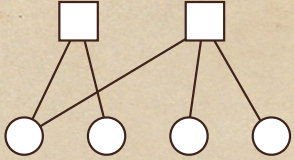
\includegraphics{Images/tanner_graph.png}}
\caption{Example of a figure caption.}
\label{fig}
\end{figure}

In Fig. \ref{fig}, we see that there are two parity nodes.

\subsection{Encoding and Generator Matrices}

\subsection{Decoding and Parity Check Matrices}

\section{Implementation of a LDPC Code in HDL}

\section{Comparison with Hamming Code HDL Implementation}

\section{Conclusion}

% \subsection{Equations}
% \begin{equation}
% a+b=\gamma\label{eq}
% \end{equation}

% Use ``\eqref{eq}'', not ``Eq.~\eqref{eq}'' or ``equation \eqref{eq}'', except at the beginning of a sentence: ``Equation \eqref{eq} is . . .''

\section*{References}

Please number citations consecutively within brackets \cite{b1}. The 
sentence punctuation follows the bracket \cite{b2}. Refer simply to the reference 
number, as in \cite{b3}---do not use ``Ref. \cite{b3}'' or ``reference \cite{b3}'' except at 
the beginning of a sentence: ``Reference \cite{b3} was the first $\ldots$''

Unless there are six authors or more give all authors' names; do not use 
``et al.''. Papers that have not been published, even if they have been 
submitted for publication, should be cited as ``unpublished'' \cite{b4}. Papers 
that have been accepted for publication should be cited as ``in press'' \cite{b5}. 
Capitalize only the first word in a paper title, except for proper nouns and 
element symbols.

For papers published in translation journals, please give the English 
citation first, followed by the original foreign-language citation \cite{b6}.

\begin{thebibliography}{00}
\bibitem{b1} G. Eason, B. Noble, and I. N. Sneddon, ``On certain integrals of Lipschitz-Hankel type involving products of Bessel functions,'' Phil. Trans. Roy. Soc. London, vol. A247, pp. 529--551, April 1955.
\bibitem{b2} J. Clerk Maxwell, A Treatise on Electricity and Magnetism, 3rd ed., vol. 2. Oxford: Clarendon, 1892, pp.68--73.
\bibitem{b3} I. S. Jacobs and C. P. Bean, ``Fine particles, thin films and exchange anisotropy,'' in Magnetism, vol. III, G. T. Rado and H. Suhl, Eds. New York: Academic, 1963, pp. 271--350.
\bibitem{b4} K. Elissa, ``Title of paper if known,'' unpublished.
\bibitem{b5} R. Nicole, ``Title of paper with only first word capitalized,'' J. Name Stand. Abbrev., in press.
\bibitem{b6} Y. Yorozu, M. Hirano, K. Oka, and Y. Tagawa, ``Electron spectroscopy studies on magneto-optical media and plastic substrate interface,'' IEEE Transl. J. Magn. Japan, vol. 2, pp. 740--741, August 1987 [Digests 9th Annual Conf. Magnetics Japan, p. 301, 1982].
\bibitem{b7} M. Young, The Technical Writer's Handbook. Mill Valley, CA: University Science, 1989.
\bibitem{b8} R.G. Gallager, Low-Density Parity-Check Codes. Cambridge, MA: MIT Press, 1963 (Sc.D. MIT, 1960).
\end{thebibliography}

\end{document}
